\section{Implementation}

\subsection{The RSBench Framework Structure}

\begin{figure}[t!]
\centering
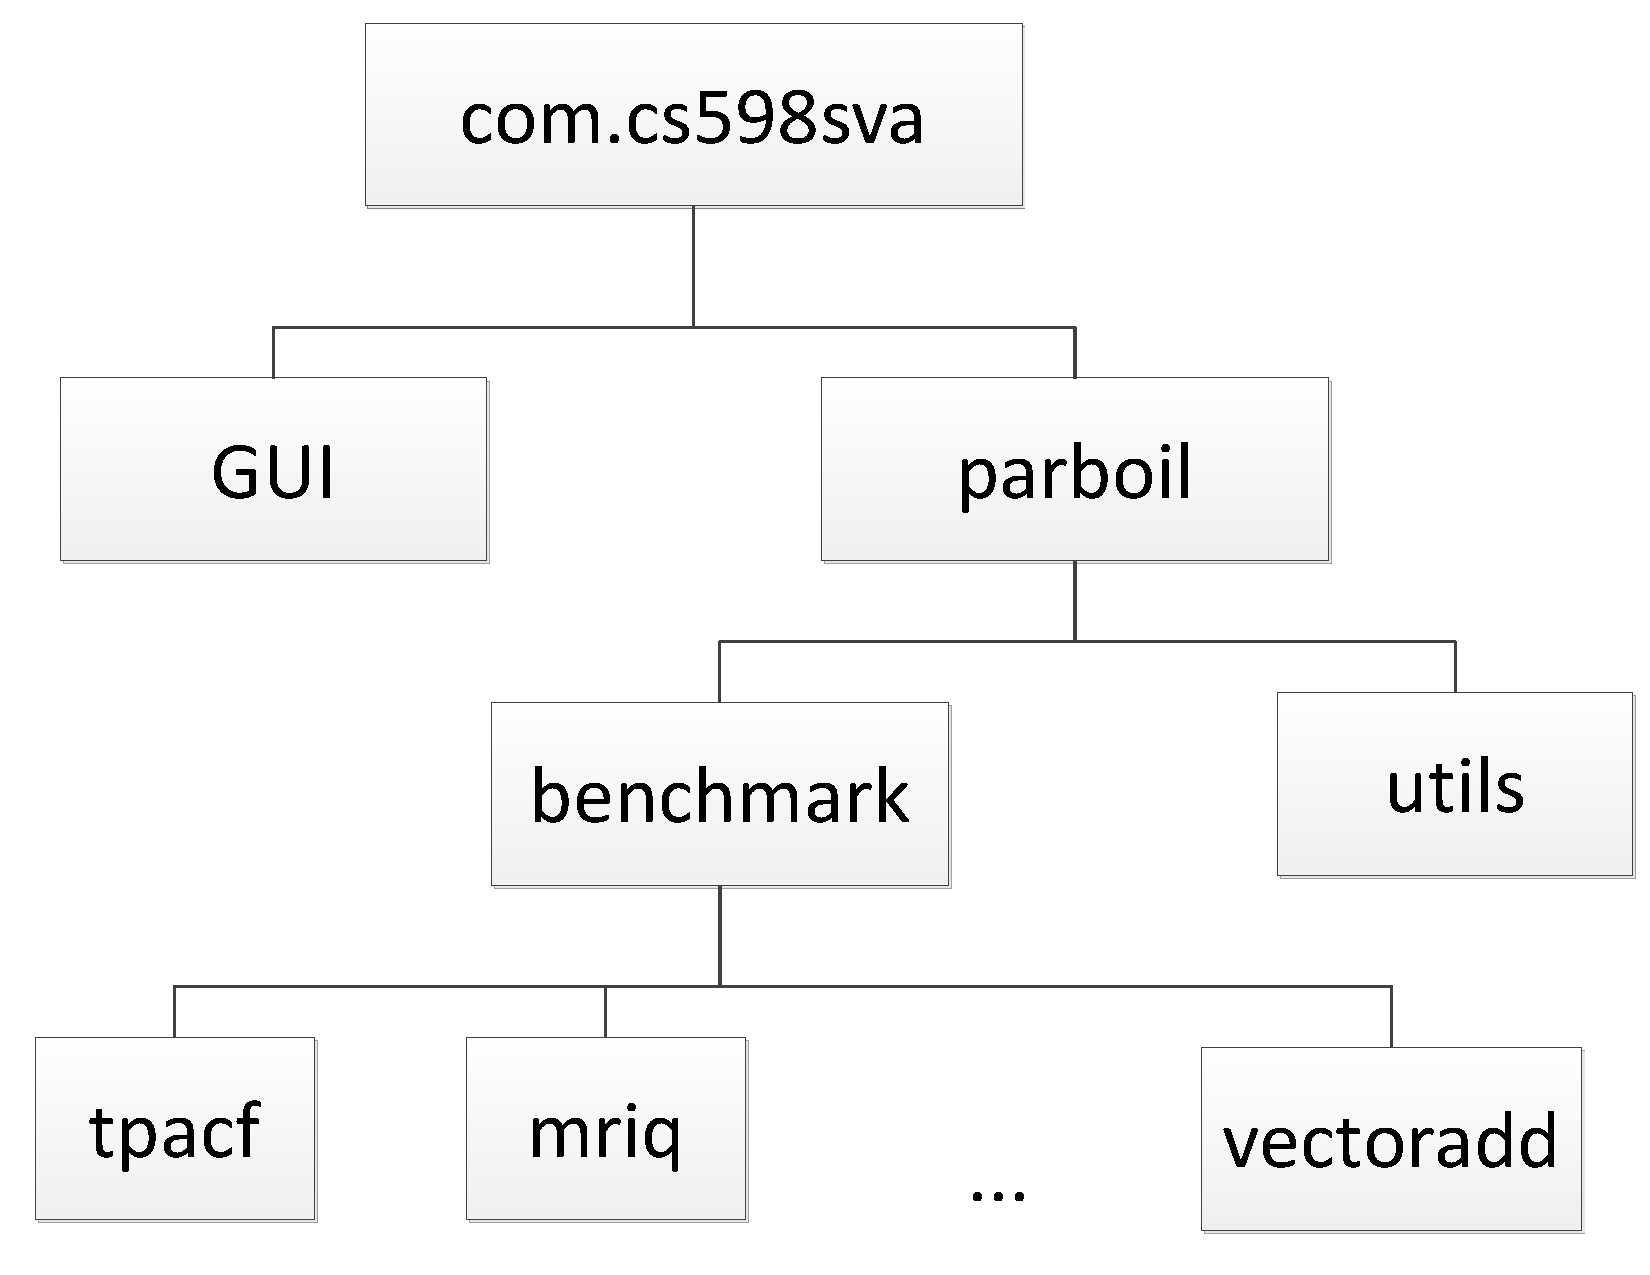
\includegraphics[scale=0.65]{figs/package_diagram.pdf}
\caption{RSBench Java package structure.}
\label{fig:package_structure}
\centering
\end{figure}


\begin{figure}[t!]
\centering
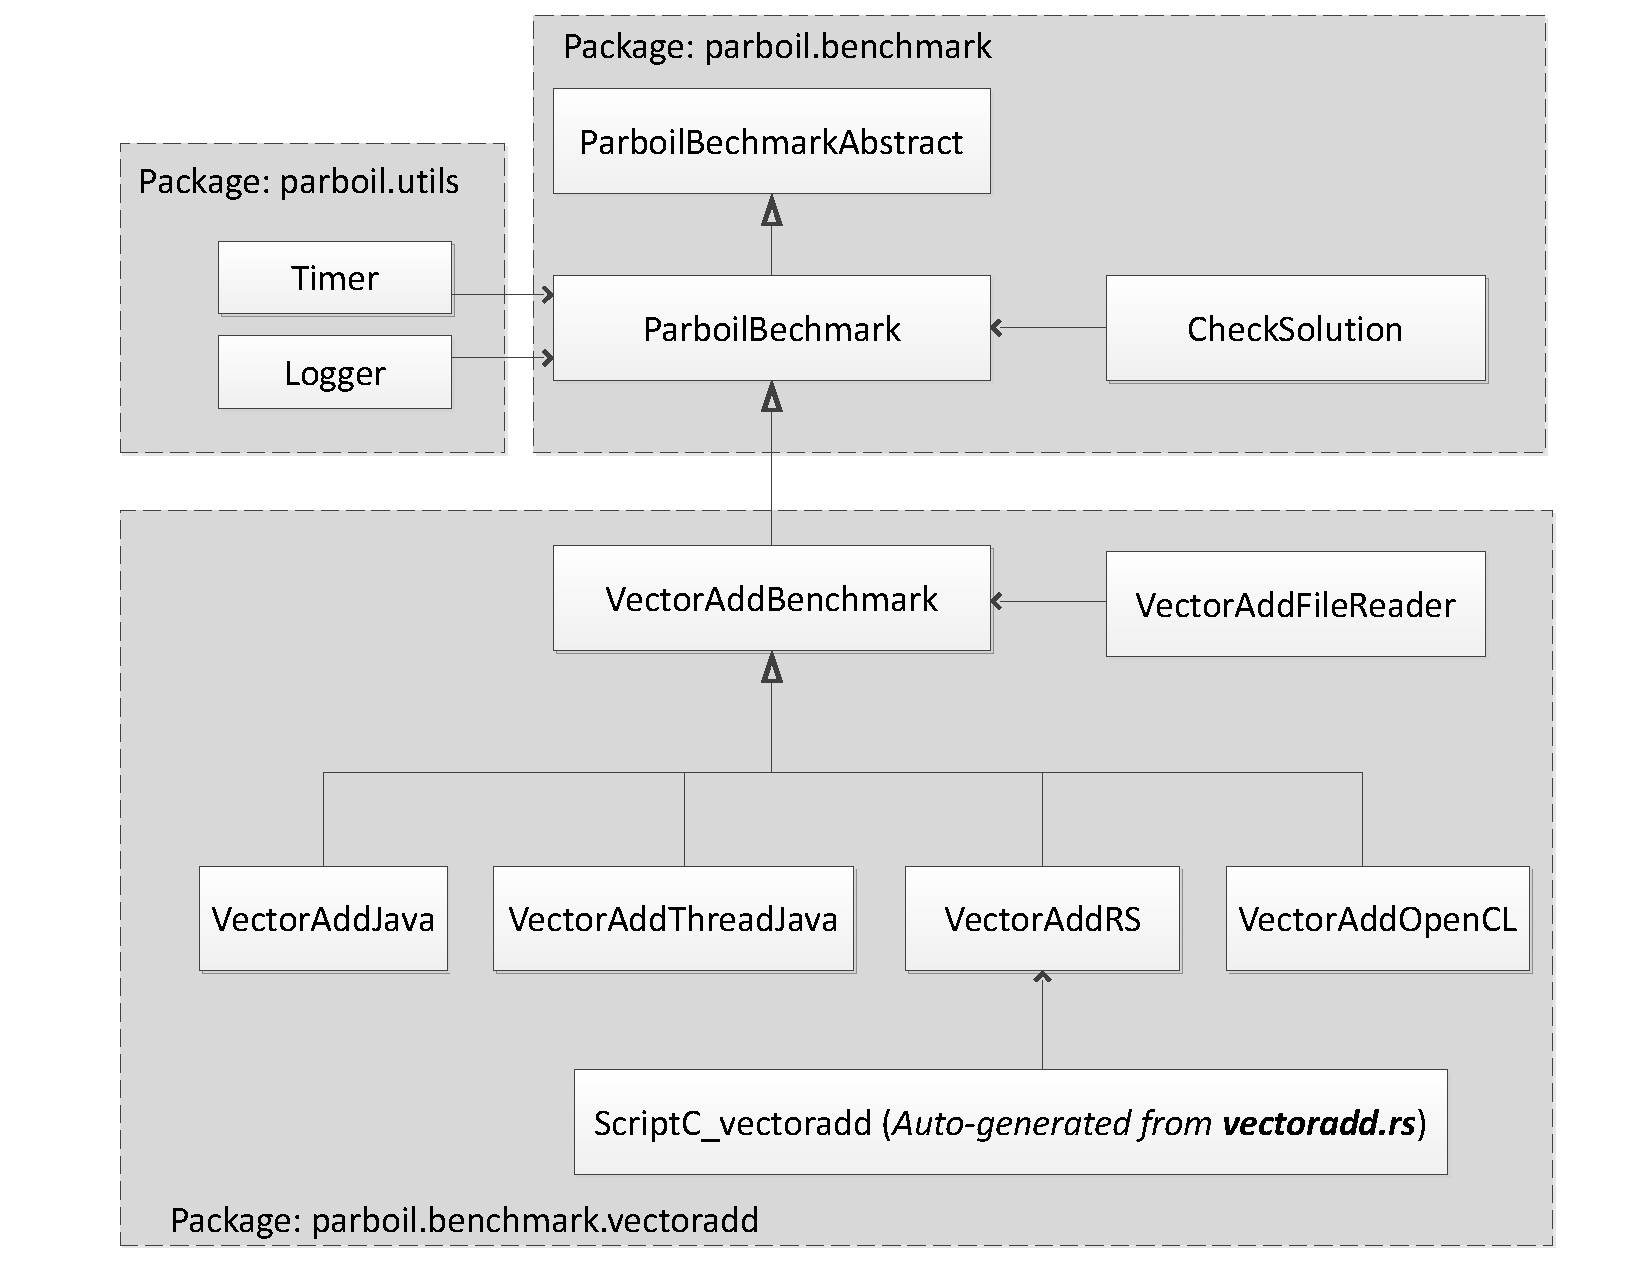
\includegraphics[scale=0.5]{figs/vectoradd_class_diagram.pdf}
\caption{Class diagram of the VectorAdd benchmark.}
\label{fig:class_diagram}
\centering
\end{figure}

In order to facilitate the development of the benchmarks, we designed a
framework, called RSBench, which contains (i) a hierarchy of the benchmarks, e.g.,
all different implementations of the same benchmark are group together, and
(ii) utilities functions that support measuring and recording the results.
Figure \ref{fig:package_structure} depicts the overview of the framework by mean
of the Java package structure. Figure \ref{fig:class_diagram} provides a closer
view at the organization of the classes related to the VectorAdd benchmark.

At a high level, we split the development of the graphical user interface (GUI),
from the development of each of the benchmarks, under the \fix{GUI} package and
the \fix{parboil} package in Figure \ref{fig:package_structure}, respectively.
At this stage, the GUI is simply to allow users to start running the benchmarks,
and to display the status of the benchmark execution, e.g., in which stage a
benchmark is running, and whether a benchmark has executed successfully or
failed at the end. In the future, more features will be added, such as
displaying the final scores of the device.

The \fix{parboil} Java package is the core of the project. In this package, we
identified the common utility functions, such as timing- and logging-related
functions, that are used across all the benchmarks. Those functions are grouped
in classes, e.g., \fix{Timer} and \fix{Logger}, and implemented in the
\fix{utils} package. Each benchmark, e,g., \fix{bfs} or \fix{cutcp}, is
implemented in a separate package under the \fix{benchmark} package.  Figure
\ref{fig:class_diagram} depicts the class diagram of the VectorAdd benchmark.
Other benchmarks have the same class structure. In order to implement a
benchmark, we just need to inherit for the \fix{ParboiBenchmark} class, which
layouts a common skeleton. For each benchmark, we have to implement a class to
read the input, for example \fix{VectorAddFileReader} class in this case. Each
computational kernel, e.g., for Java, threaded Java, RenderScript, or OpenCL, is
implemented in a separate class, e.g., \fix{VectorAddJava},
\fix{VectorAddThreadedJava}, \fix{VectorAddRS}, or \fix{VectorAddOpenCL},
respectively. These classes inherit from the parent class of the benchmark,
which is the \fix{VectorAddBenchmark} in this case. This hierarchical design
maximize the code reuse between benchmarks, and between computation kernel.  It
also allows for a consistent interface to run the benchmarks.


\subsection{Utility Classes}
\subsection{Timer}
The \fix{Timer} class is an important utility in our benchmark. It
determines the accuracy and flexibility of our measurement. The \fix{Timer}
class utilizes Android's \fix{SystemClock}, which provides real-time clock at
nanosecond resolution. Each \fix{Timer} object consists of a dynamic list of
\fix{TimerElement} objects. Each \fix{TimerElement} object is a measure of a
particular execution segment, e.g., allocation time, setup time, and compute
time. In order to create a new \fix{TimerElement}, we just need to invoke the
\fix{Timer.start(category, message)} method at the beginning of the execution
segment we wish to measure (here category is a user defined category such as
``Compute'' or ``Setup'', while message is a message that further refines the
category such as ``Allocating temporary datastructures''). At the end of the
execution segment, we need to invoke the \fix{Time.stop()} method. The
time-stamp and elapsed time will be automatically computed and recorded.

If a benchmark is run multiple times, for example, we run the compute part of
the implementation 5 times in our currently analysis, then we take the minimum
amount of time for each block. While this does hide some overhead (the JIT
compilation in Java, for example) it does reflect the maximum performance one
can achieve for each implementation.

\subsection{Time Database}

Unlike Parboil, which outputs the times to {\tt stdout}, we output our data into
a SQLite database.  This affords us a few things.  First, since data is
outputted in the specified columns, we do not have to re-parse the output data.
Second, timing information can be shared easily by copying the database.
Finally, we can store more than just timing information -- for example we also
store which machine the time has been taken on as well as which runtime is being
used.  Since writing to flash is extensive, all timing data is stored in memory
and after the benchmark has run it is inserted into the database. 

\subsection{Load/Power Profiler}

Since Android does not offer a way to capture processor usage information
programatically, we use the Trepn tool by Qualqomm to capture the data for us
and save it into a {\tt csv} file.   Trepn, which is limited to Qualcomm based
chipsets, reads internal processor counters as well as power rail information,
both of which are not otherwise available programatically.  We set Trepn to read
the counters every $100ms$ and measure the load and power usage seperatly to
decrease the overhead of the profiler.  To reduce overhead, Trepn measure the
processor usage information every $100ms$, both the frequency and the load are
measured sequentially, we therefore need to correct that when parsing the {\tt
csv} file.

First, we parse each processor reading along with the time stamp for reading the
file.  Next, we interpolate the measured data (we use linear interpolant) and
evaluate the interpolant at the application state times (these are the times
Trepn recieved a signal from our application and correspond to timed blocks of
code).  We then multiply the load by the frequency, and rescale all the CPU and
GPU data (we perform the rescaling on the CPU and GPU seperatly).  Trepn can
have measurment errors, resulting in infinite numbers.  To make sure that these
do not skew the plots, we clip the range of possible processor reading to be
between 1 and the the $0.99$th quantile of the data.  While efforts have
been taken to reduce the profiler's overhead, it still ocupies around a
$10\%$ overhead.


\subsection{Computational Kernels}

\begin{table}[h]\small
\centering
\begin{tabular}{ | l | c |}
    \hline 
    Language      & Line Count \\ \hline
    Java          & 7549       \\ \hline
    RenderScript  & 1000       \\ \hline
    JNI/C++       & 2048       \\ \hline
    OpenCL        & 480        \\ \hline
\end{tabular}
\caption{RSBench project line count breakdown.}
\label{table:breakdown}
\end{table}

Table~\ref{table:breakdown} shows the numbers of line-of-code (LOC) broken down
into different types of programming languages in the RSBench project. The next
sub-sections describe the process of implementing different types of computational
kernels for each benchmark.

\subsection{RenderScript Kernels}
%This section describes the general steps to write a computation kernel in
%RenderScript for our benchmark.

By design, each RenderScript kernel produces an \textit{element} of the output.
It is up to developers to define the granularity of an element. For example, in
the VectorAdd benchmark, an output element can be one, or two, or three array
elements of the output vector. This granularity essentially determines the
parallelism of the written RenderScript code. In our benchmarks, we select the
finest granularity of the output element, e.g., one array element in this case,
to implement our RenderScript kernel.

In order to support this model, the RenderScript framework provides APIs to (i)
define the type of \fix{Element} for both input and output of RenderScript
kernels, and (ii) pack \fix{Element}s into \fix{Allocation}, which is the data
structure that is used to pass data back and forth between regular Java code and
RenderScript code.

A significant effort of our work is to determine efficient ways to convert input
data from original structure to the \fix{Allocation} structure with appropriate
\fix{Element} type. This conversion is also reflected at runtime through the
\textit{setup} time category of RenderScript execution.

After data has been packed into \fix{Allocation} objects, we move to write
RenderScript code in C99 format. The code needs to be placed in a specific file
with the $.rs$ extension and a proper header, so that the Android Development
Tools (ADT) can automatically generate a wrapper Java class for it. The
auto-generated Java class provides interfaces to invoke the RenderScript code
from Java code.

\subsection{Native Kernels}

The Android operating system requires that C, OpenMP, and OpenCL kernels have to
be invoked through Java Native Interface (JNI).  The C and OpenMP versions of
the code have been taken from Parboil with minimal modifications.  The code is
wrapped via JNI so it is callable from within Java.

The OpenCL kernels are lifted from the parboil benchmark suite with no
modifications.  We use the \fix{base} implementation of OpenCL --- this a
platform agnostic unoptimized implementation.  Unlike the Parboil benchmark
suite, we write the OpenCL host code using the C++ OpenCL API, this simplifies
some of the code and affords us more code reuse oportunities.

To allow devices with no OpenCL support to make use of the C and OpenMP
implementations, we generate 3 libraries (one for C, OpenMP, and OpenCL).  Each
library is then loaded and called from with its class implementation.
